\documentclass{assignment}

\course{ECO 120-04}
\name{Lucas Reddinger}
\date{Friday 9 December 2022}
\doctitle{Assignment 9 Solutions}

\begin{document}
\RaggedRight

\beginsolutions{}

Suppose that the U.S.~economy is initially in long-run equilibrium, producing its potential output $Y_p$, as depicted directly below.

\section{Recessions and expansions}

\begin{enumerate}
\item Please define a recessionary period using actual output $Y$ and potential output $Y_p$.
\begin{solution}
$Y<Y_p$ or $Y-Y_p<0$ (notice that these are equivalent statements).
\end{solution}
\item Please define an expansionary period using actual output $Y$ and potential output $Y_p$.
\begin{solution}
$Y>Y_p$ or $Y-Y_p>0$ (notice that these are equivalent statements).
\end{solution}
\item Please define the output gap using actual output $Y$ and potential output $Y_p$.
\begin{solution}
The output gap is $\frac{Y-Y_p}{Y_p}\times100\%$.
\end{solution}
\item Please define a recessionary period using the output gap.
\begin{solution}
We know that $Y-Y_p<0$. We can multiply both sides by $\frac{100\%}{Y_p}$ to obtain $\frac{Y-Y_p}{Y_p}\times100\%<0$.

That is, the output gap is negative.
\end{solution}
\item Please define an expansionary period using the output gap.
\begin{solution}
We know that $Y-Y_p>0$. We can multiply both sides by $\frac{100\%}{Y_p}$ to obtain $\frac{Y-Y_p}{Y_p}\times100\%>0$.

That is, the output gap is positive.
\end{solution}
\end{enumerate}

\section{An economy during a recessionary period\label{sec:recession}}

Please graph an economy in a recessionary period using the aggregate supply and demand model.

\begin{enumerate}

\item Begin by drawing and labeling axes.

\item Draw and label an aggregate demand (AD) and short-run aggregate supply (SRAS) curves.

\item Label the aggregate price level $P^*_0$ and the actual output level $Y^*_0$.

\begin{solution}
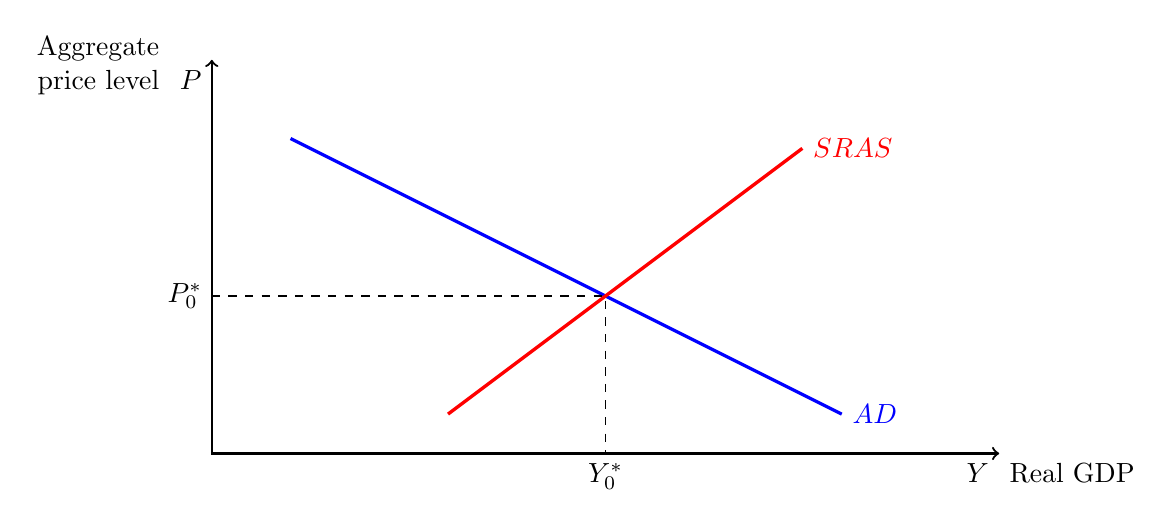
\begin{tikzpicture}[scale=0.5]
\draw[thick,<->] (0,10) node[below left,label={[align=right]left:Aggregate\\price level\\ }] {$P$} --(0,0)--(20,0) node[below left,label=right:Real GDP]{$Y$};
\draw[very thick,blue] (2,8)--(16,1) node[right]{$\text{AD}$};
\draw[very thick,red] (6,1)--(15,7.75) node[right]{$\text{SRAS}$};
\draw[dashed] (0,4) node[left]{$P^*_0$} --(10,4) --(10,0)node[below]{$Y^*_0$};
\end{tikzpicture}
\end{solution}

\item In a recession, is potential output $Y_p$ above or below actual output $Y^*_0$?

\begin{solution}
Above.
\end{solution}

\item Add a long-run aggregate supply (LRAS) curve to your graph, and label $Y_p$.

\begin{solution}
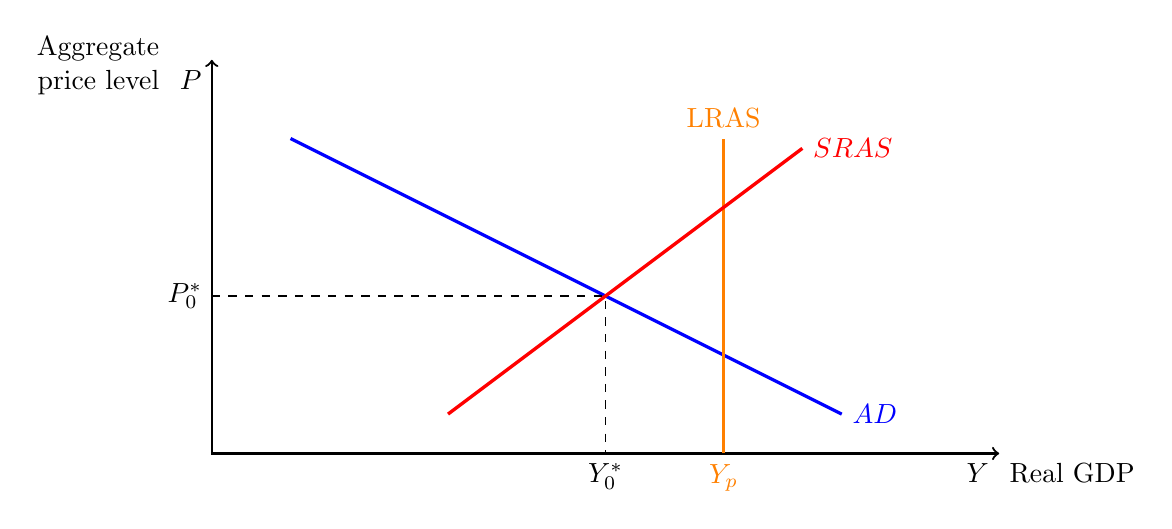
\begin{tikzpicture}[scale=0.5]
\draw[thick,<->] (0,10) node[below left,label={[align=right]left:Aggregate\\price level\\ }] {$P$} --(0,0)--(20,0) node[below left,label=right:Real GDP]{$Y$};
\draw[very thick,blue] (2,8)--(16,1) node[right]{$\text{AD}$};
\draw[very thick,orange] (13,0) node[below]{$Y_p$}--(13,8) node[above]{LRAS};
\draw[very thick,red] (6,1)--(15,7.75) node[right]{$\text{SRAS}$};
\draw[dashed] (0,4) node[left]{$P^*_0$} --(10,4) --(10,0)node[below]{$Y^*_0$};
\end{tikzpicture}
\end{solution}

\end{enumerate}

\section{An economy during an expansionary period\label{sec:expansion}}

Please graph an economy in an expansionary period using the aggregate supply and demand model.

\begin{enumerate}

\item Begin by drawing and labeling axes.

\item Draw and label an aggregate demand (AD) and short-run aggregate supply (SRAS) curves.

\item Label the aggregate price level $P^*_0$ and the actual output level $Y^*_0$.

\begin{solution}
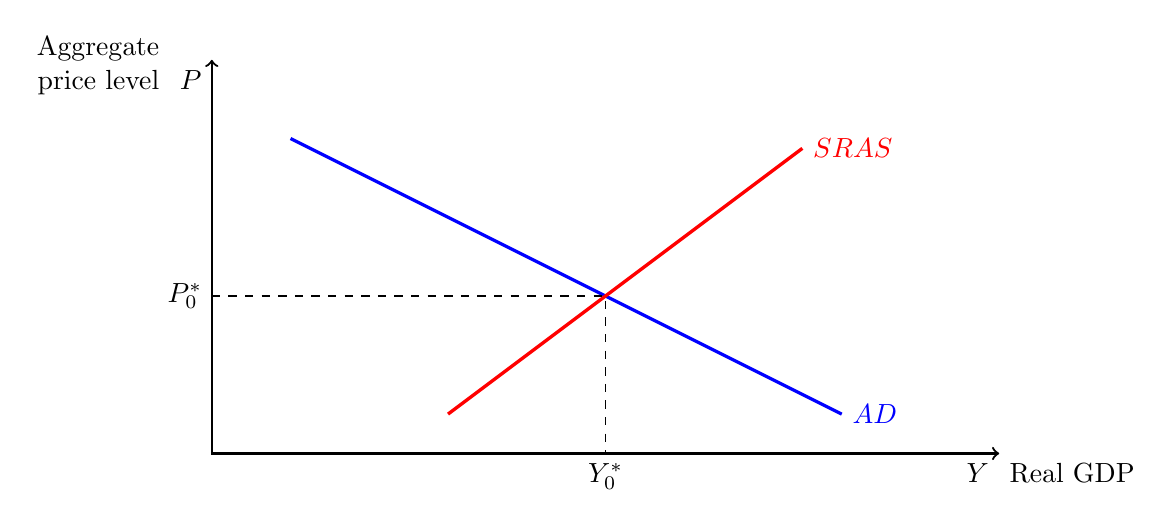
\begin{tikzpicture}[scale=0.5]
\draw[thick,<->] (0,10) node[below left,label={[align=right]left:Aggregate\\price level\\ }] {$P$} --(0,0)--(20,0) node[below left,label=right:Real GDP]{$Y$};
\draw[very thick,blue] (2,8)--(16,1) node[right]{$\text{AD}$};
\draw[very thick,red] (6,1)--(15,7.75) node[right]{$\text{SRAS}$};
\draw[dashed] (0,4) node[left]{$P^*_0$} --(10,4) --(10,0)node[below]{$Y^*_0$};
\end{tikzpicture}
\end{solution}

\item In an expansion, is potential output $Y_p$ above or below actual output $Y^*_0$?

\begin{solution}
Below.
\end{solution}

\item Add a long-run aggregate supply (LRAS) curve to your graph, and label $Y_p$.

\begin{solution}
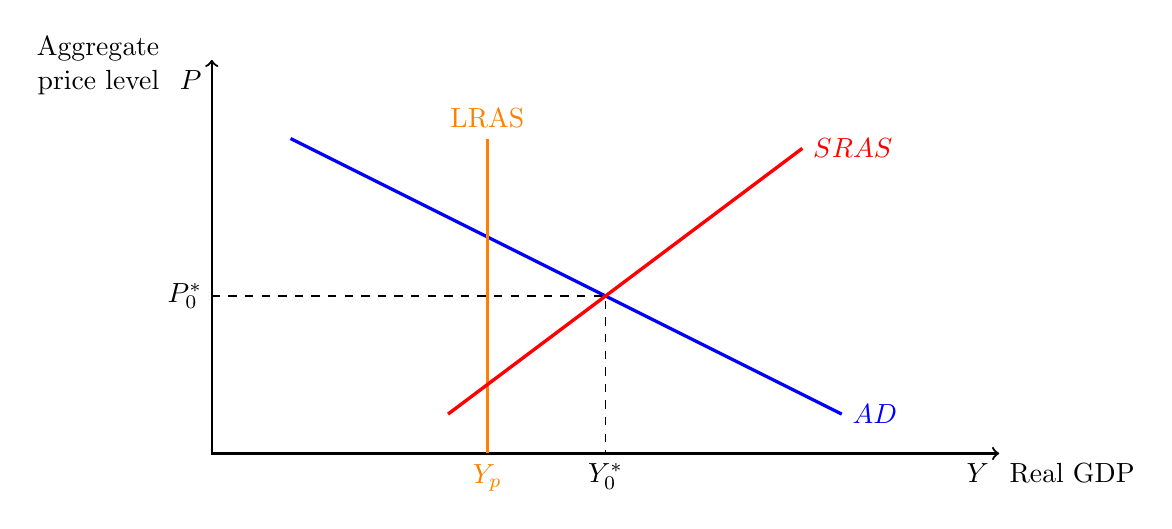
\begin{tikzpicture}[scale=0.5]
\draw[thick,<->] (0,10) node[below left,label={[align=right]left:Aggregate\\price level\\ }] {$P$} --(0,0)--(20,0) node[below left,label=right:Real GDP]{$Y$};
\draw[very thick,blue] (2,8)--(16,1) node[right]{$\text{AD}$};
\draw[very thick,orange] (7,0) node[below]{$Y_p$}--(7,8) node[above]{LRAS};
\draw[very thick,red] (6,1)--(15,7.75) node[right]{$\text{SRAS}$};
\draw[dashed] (0,4) node[left]{$P^*_0$} --(10,4) --(10,0)node[below]{$Y^*_0$};
\end{tikzpicture}
\end{solution}

\end{enumerate}

\section{The short-run and the long-run}

\begin{enumerate}

\item What characterizes the short-run in the aggregate supply and demand (AS and AD) model?

\begin{solution}
Wages are sticky in the short-run. Wages are flexible in the long-run.
\end{solution}

\item Which curve shifts as nominal wages change?

\begin{solution}
The SRAS curve.
\end{solution}

\item In which direction does the curve shift \emph{when nominal wages increase}?

\begin{solution}
The SRAS curve shifts in (or left).
\end{solution}

\item In which direction does the curve shift \emph{when nominal wages decrease}?

\begin{solution}
The SRAS curve shifts out (or right).
\end{solution}

\item In long-run equilibrium, $Y=Y_p$. Revisit \cref{sec:recession}, with \emph{an economy in a recessionary period}. Suppose that wages adjust so that the economy returns to long-run equilibrium. Consider what shift would be necessary to make $Y=Y_p$. Graph this shift, and label the new price level $P^*_1$ and new actual output level $Y^*_1$. Did wages increase or decrease?

\begin{solution}
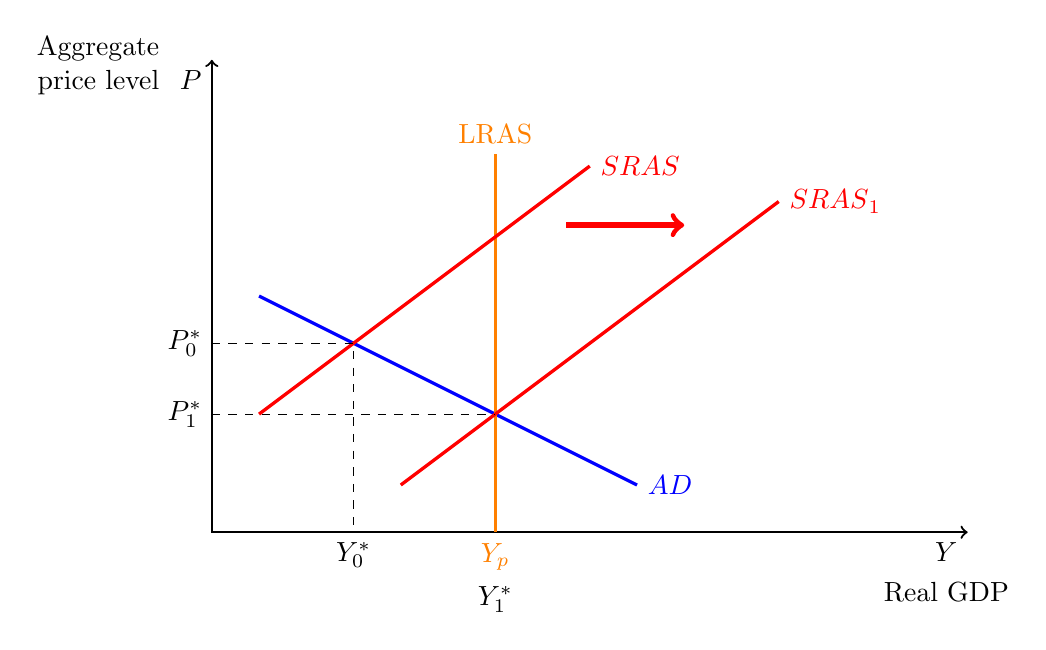
\begin{tikzpicture}[scale=0.6]
\draw[thick,<->] (0,10) node[below left,label={[align=right]left:Aggregate\\price level\\ }] {$P$} --(0,0)--(16,0) node[below left,label=below:Real GDP]{$Y$};
\draw[very thick,blue] (1,5)--(9,1) node[right]{$\text{AD}$};
\draw[very thick,orange] (6,0) node[below]{$Y_p$}--(6,8) node[above]{LRAS};
\draw[very thick,red] (1,2.5)--(8,7.75) node[right]{$\text{SRAS}$};
\draw[very thick,red] (4,1)--(12,7) node[right]{$\text{SRAS}_1$};
\draw[dashed] (0,4) node[left]{$P^*_0$} --(3,4) --(3,0)node[below]{$Y^*_0$};
\draw[dashed] (0,2.5) node[left]{$P^*_1$}--(6,2.5);
\node[below,yshift=-16pt] at (6,0) {$Y^*_1$};
\draw[line width=2pt,->,red] (7.5,6.5)--(10,6.5);
\end{tikzpicture}

Wages decreased, causing this rightward shift of the SRAS curve. (When labor is cheaper, firms are willing to produce more output at any given price.)

\vspace{-8pt}
\end{solution}

\item In long-run equilibrium, $Y=Y_p$. Revisit \cref{sec:expansion}, with \emph{an economy in an expansionary period}. Suppose that wages adjust so that the economy returns to long-run equilibrium. Consider what shift would be necessary to make $Y=Y_p$. Graph this shift, and label the new price level $P^*_1$ and new actual output level $Y^*_1$. Did wages increase or decrease?

\begin{solution}
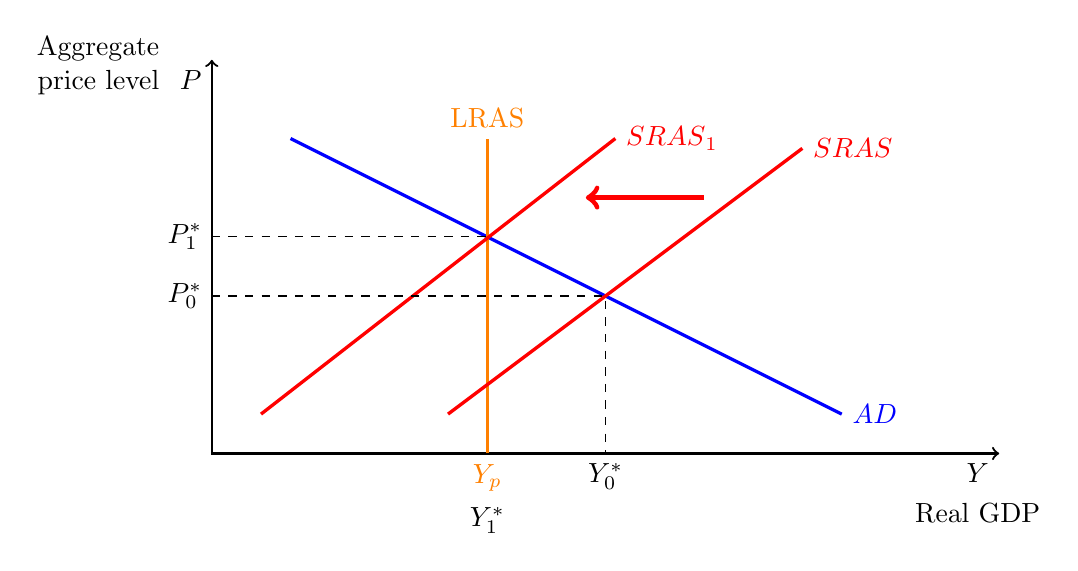
\begin{tikzpicture}[scale=0.5]
\draw[thick,<->] (0,10) node[below left,label={[align=right]left:Aggregate\\price level\\ }] {$P$} --(0,0)--(20,0) node[below left,label=below:Real GDP]{$Y$};
\draw[very thick,blue] (2,8)--(16,1) node[right]{$\text{AD}$};
\draw[very thick,orange] (7,0) node[below]{$Y_p$}--(7,8) node[above]{LRAS};
\draw[very thick,red] (6,1)--(15,7.75) node[right]{$\text{SRAS}$};
\draw[very thick,red] (1.25,1)--(10.25,8) node[right]{$\text{SRAS}_1$};
\draw[dashed] (0,4) node[left]{$P^*_0$} --(10,4) --(10,0)node[below]{$Y^*_0$};
\draw[dashed] (0,5.5) node[left]{$P^*_1$}--(7,5.5);
\node[below,yshift=-16pt] at (7,0) {$Y^*_1$};
\draw[line width=2pt,->,red] (12.5,6.5)--(9.5,6.5);
\end{tikzpicture}

Wages increased, causing this leftward shift of the SRAS curve. (When labor is more expensive, firms will reduce their output at any given price.)
\end{solution}

\end{enumerate}

\end{document}
